%----------------------------------------
% Preamble to set up the document
%----------------------------------------
\documentclass{article}

% set up packages (you shouldn't need to touch this)
\usepackage{amsmath}
\usepackage{amssymb}
\usepackage{graphicx}  % required to insert images
\usepackage{hyperref}  % for hyperlinks
\usepackage[svgnames]{xcolor}  % to change hyperlink colors
\colorlet{linkcolour}{DarkBlue}
\hypersetup{colorlinks=true, linkcolor=linkcolour, citecolor=linkcolour, urlcolor=linkcolour,}

% Margins
\topmargin=-0.45in
\evensidemargin=0in
\oddsidemargin=0in
\textwidth=6.5in
\textheight=9.0in
\headsep=0.25in

% use a sans serif font
\renewcommand{\familydefault}{\sfdefault}

%----------------------------------------
% Step 1: Edit the lecture title
%----------------------------------------
\title{
Lecture 7: Regression \\  % Lecture title
Modeling Social Data, Spring 2019 \\   % Course title
Columbia University                    % School
}

%----------------------------------------
% Step 2: Edit your name and the date
%----------------------------------------
\author{Vatsala Swaroop (vs2671)}                     % Scribe's name
\date{March 13, 2019}                % Lecture date

\begin{document}

\maketitle


%----------------------------------------
% Step 3:
% Rename uni.tex to match your uni,
% edit the filename accordingly below,
% and put your notes in this file
%----------------------------------------
%----------------------------------------
% Write your notes here
%----------------------------------------

\section{Continuation of Reproducibility, Replication Lecture}

The Lecture begins with a continued overview into what we should do - 
\begin{itemize}
  \item Read the literature - It is important to know what work has already been done. This might also help you think and understand about the problem more.
  \item Formulate your study
  \item Run a simple pilot - a basic version is run to get initial results. This can result in revisions in the study
  \item Analyze the results
  \item Revise your study (null != nil)
  \item Do a power calculation (think about effect size here - reference to homework 2)
  \item Pre-register your plans
  \item Run your study
  \item Create a reproducible report - important for others to check the work
  \item Think critically about results
  \item Disclose everything you did - this also includes details around data collection
\end{itemize}
\bigskip
Next, Professor Jake gives an example of his own research, findings and interpretation. We see an experiment revolving around the probability to win if an item is picked. Multiple tests are run for significance of difference in willingness to pay between the two items.
\\
\\
In order to collect the data, they used Mechanical Turk - a platform that typically allows people to earn small amounts of money for tasks/surveys completed. It was found by him that the average responses by a random set of people on Turk were not typically different from how someone who knew about the subject would respond.
\\
\\
We also see a brief overview of the data file they get back. Typically, a lot of data is collected and can be used for different purposes -
\\
eg. We revisit the boulder experiment covered two lectures before. Data like when they saw start boulder, timestamps so that they can check for bots and filter them out
\\
\\
The steps he has followed closely match the description of what we should do stated above. They can be briefly summarized as -
\\
\\
Data collection $\rightarrow$ Run pilot $\rightarrow$ See Rmd and finalize result  $\rightarrow$ Study to check $\rightarrow$ Analysis and summary of findings

\subsection{Brief revisit to standard error and deviation}
For a sample size of 10 people, we compute the average value for a quantity
\\
\\
Standard error - variation in the average decreases with more samples
\\
\\
Standard deviation - Measure of uncertainity in the population
\begin{equation*}
  \sigma = \frac{\sigma_x}{N^{1/2}} 
\end{equation*}
\\
The standard deviation graph is relevant for effect size. If means are different but the variation overlaps a lot, then that is not very significant.


\section{Regression}

Regression analysis basically refers to using the available data to infer relationships from variables and predict future outcomes.
\subsection{Goals}
The primary goals of regression analysis are to -
\begin{itemize}
    \item 
    Predict future outcomes
    \item Explain associations between predictors and outcomes
    \item
    Describe or summarize outcomes under different conditions
\end{itemize}
An example of regression analysis would be SAT scores for Asian vs Hispanic students.
\\
\subsection{Prediction problem}
We basically want to find a function f whose output matches the data well such that
\begin{equation*}
  y_i = f(x_i)
\end{equation*}
Here, y is the output/outcome vector represented by 
$$\begin{bmatrix} 
    y_{1} \\
    \vdots \\
    y_{N} 
\end{bmatrix}$$
\\
And x is the input vector such that there are n training samples of d dimensions/features each
$$\begin{bmatrix} 
    x_{11} & \dots & x_{1d} \\
    \vdots \\
    x_{n1} &        & x_{nd} 
\end{bmatrix}$$

\subsection{Loss Function}
To arrive at our desired function mapping f(x), we define a loss function. Our goal is to \textbf{minimize this loss function}
\\
\\
A reasonable choice of loss function is Least squares error
$$L_i[f]=\frac{1}{N}\sum_{1}^{N}(y_i-f(x_i))^2$$
Another choice is the absolute loss function $$L_i[f]=\frac{1}{N}\sum_{1}^{N}|y_i-f(x_i)|$$
\\
Here $y_i$ is actual outcome and $f(x_i)$ is the predicted outcome.

\subsection{Maximum Likelihood Interpretation}
\textbf{Assumption}: We imagine that the data is generated by
\begin{equation*}
y_i = f(x_i) + \epsilon_i
\end{equation*}
such that $\epsilon_i \sim N(0, \sigma^2)$
\\
We can then calculate the likelihood of seeing the observed data D as -
\begin{equation*}
p(D|f) =  \prod_{i=1}^{N}p(\epsilon_i | f) 
= (\frac{1}{\sqrt{2\pi\sigma^2}})^N \prod_{i=1}^{N}e^{-\frac{1}{2\sigma^2}(y_i - f(x_i))^2} 
\end{equation*}
\\
\textbf{Observe} : We have assumed independence here.
\\
What we basically want to find is under what function f is the probability of the observed data maximized.
\\
\\
This is given by
\\
\begin{align*}
f^{*} = \operatorname*{argmax}_f p(D|f) 
\end{align*}
where $f^{*}$ Maximum Likelihood Solution.
\\
\\


\subsection{Maximum Log Likelihood and relation to Least square error}
Since it is difficult to calculate in the product form stated above, we take a log to deal with the products! It is okay to do this because of the monotonically increasing nature of log function.
\\
Then log of maximum likelihood becomes -

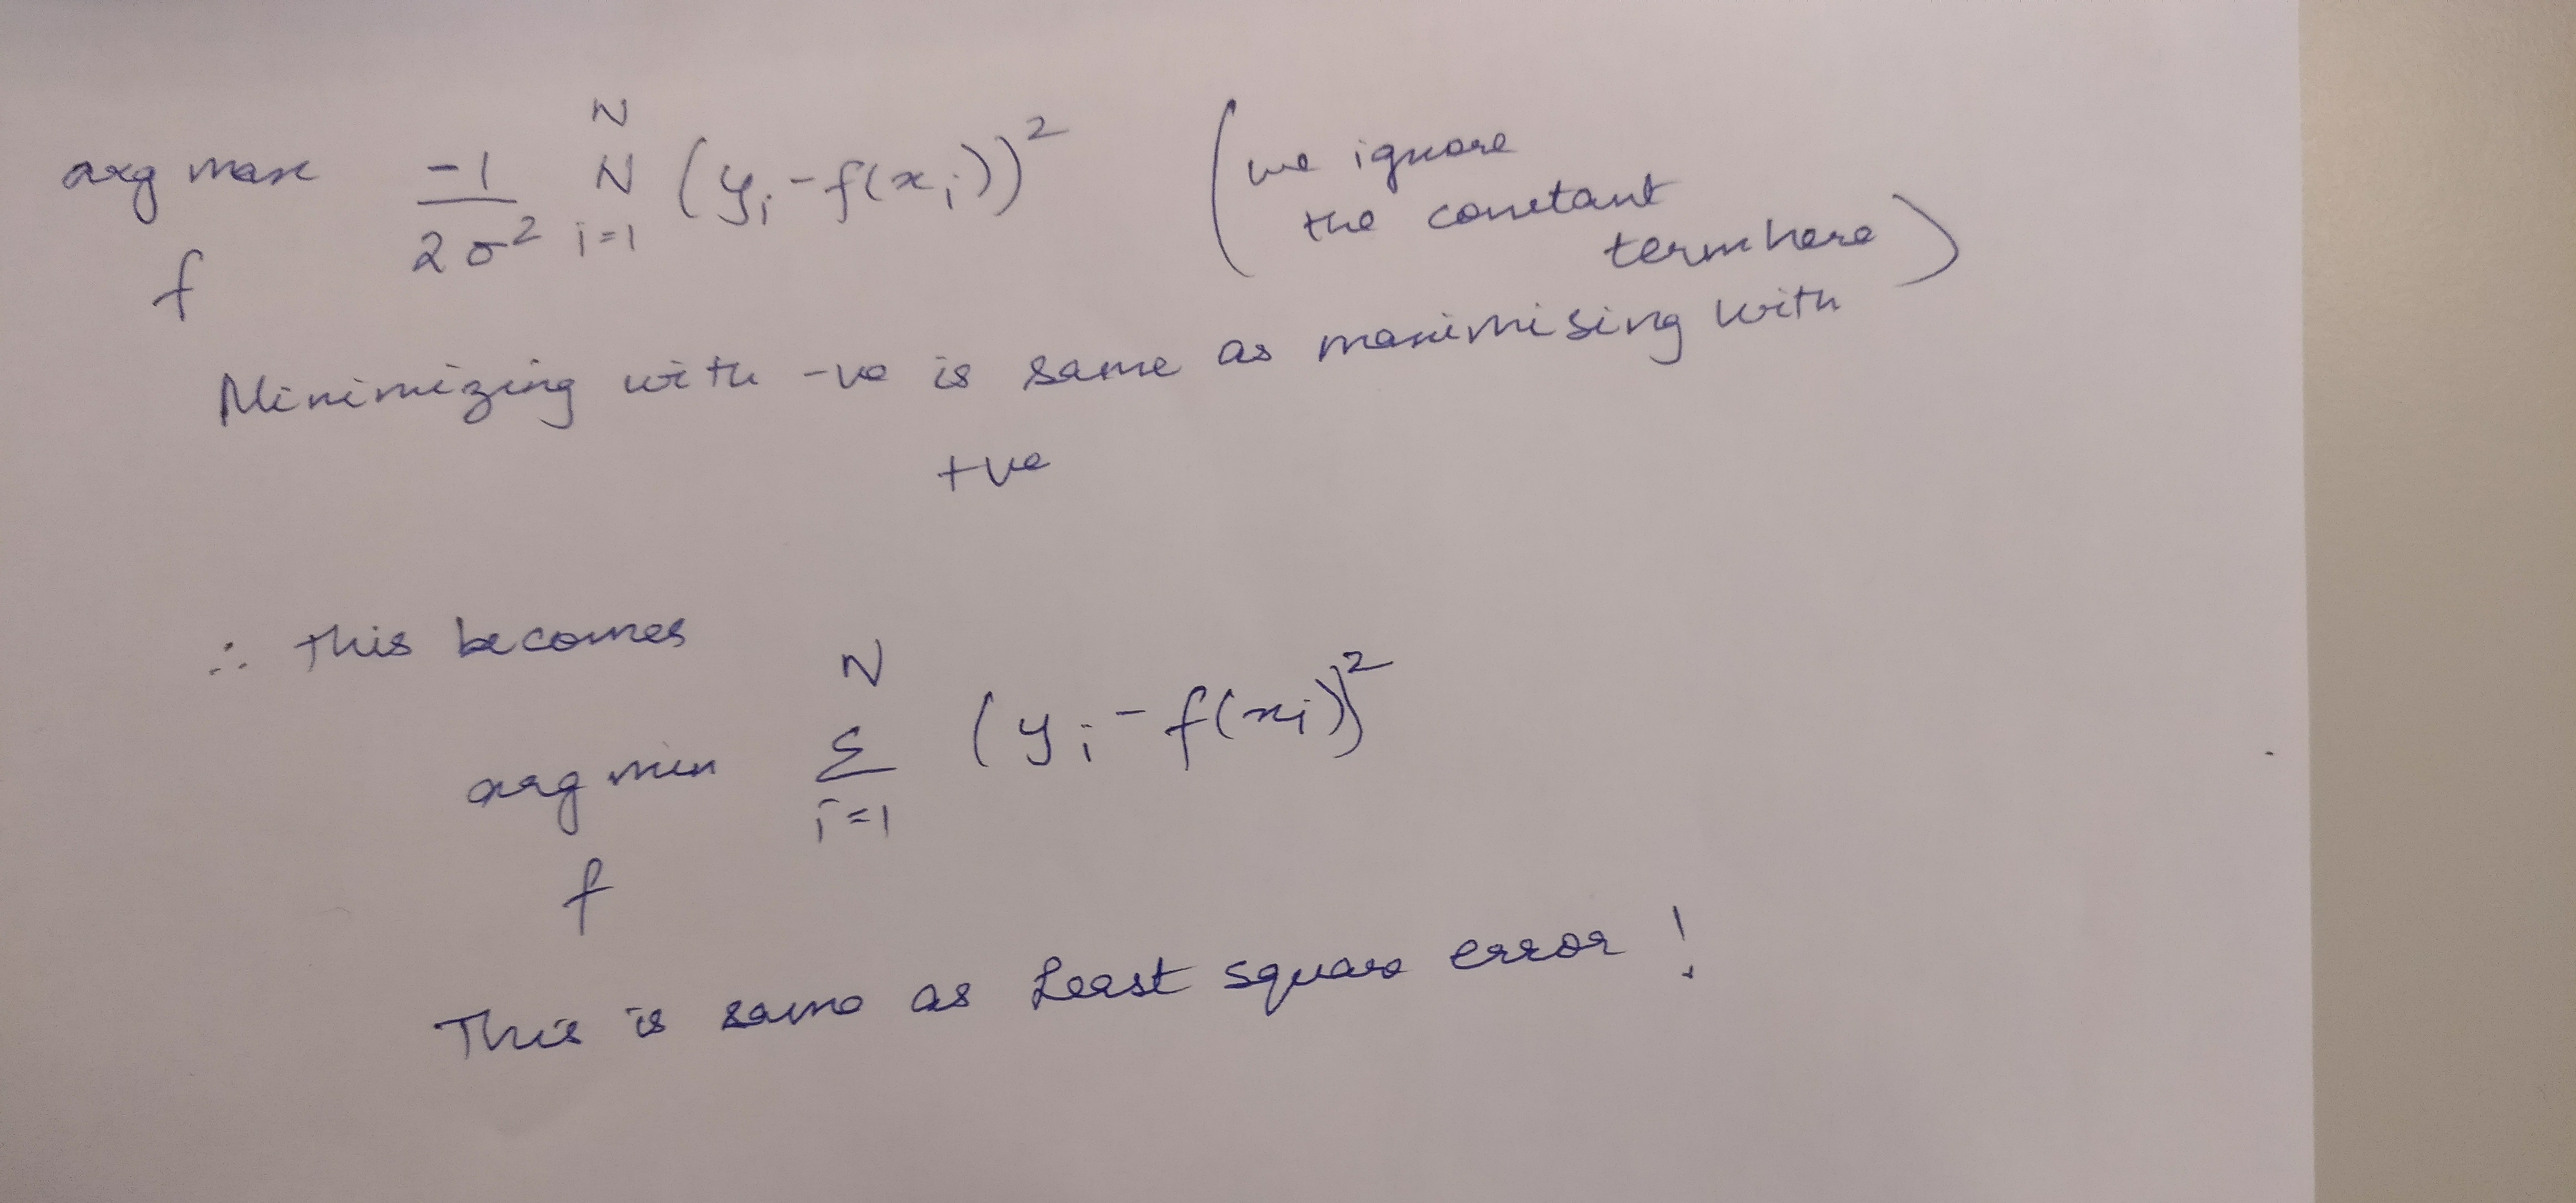
\includegraphics[width=15cm,height = 8cm]{figures/log_mle.jpg}
\\
\\
Hence, we can achieve the Maximum Likelihood Solution by solving Least Squared Error.\\

\subsection{Computing Desired weight vector}
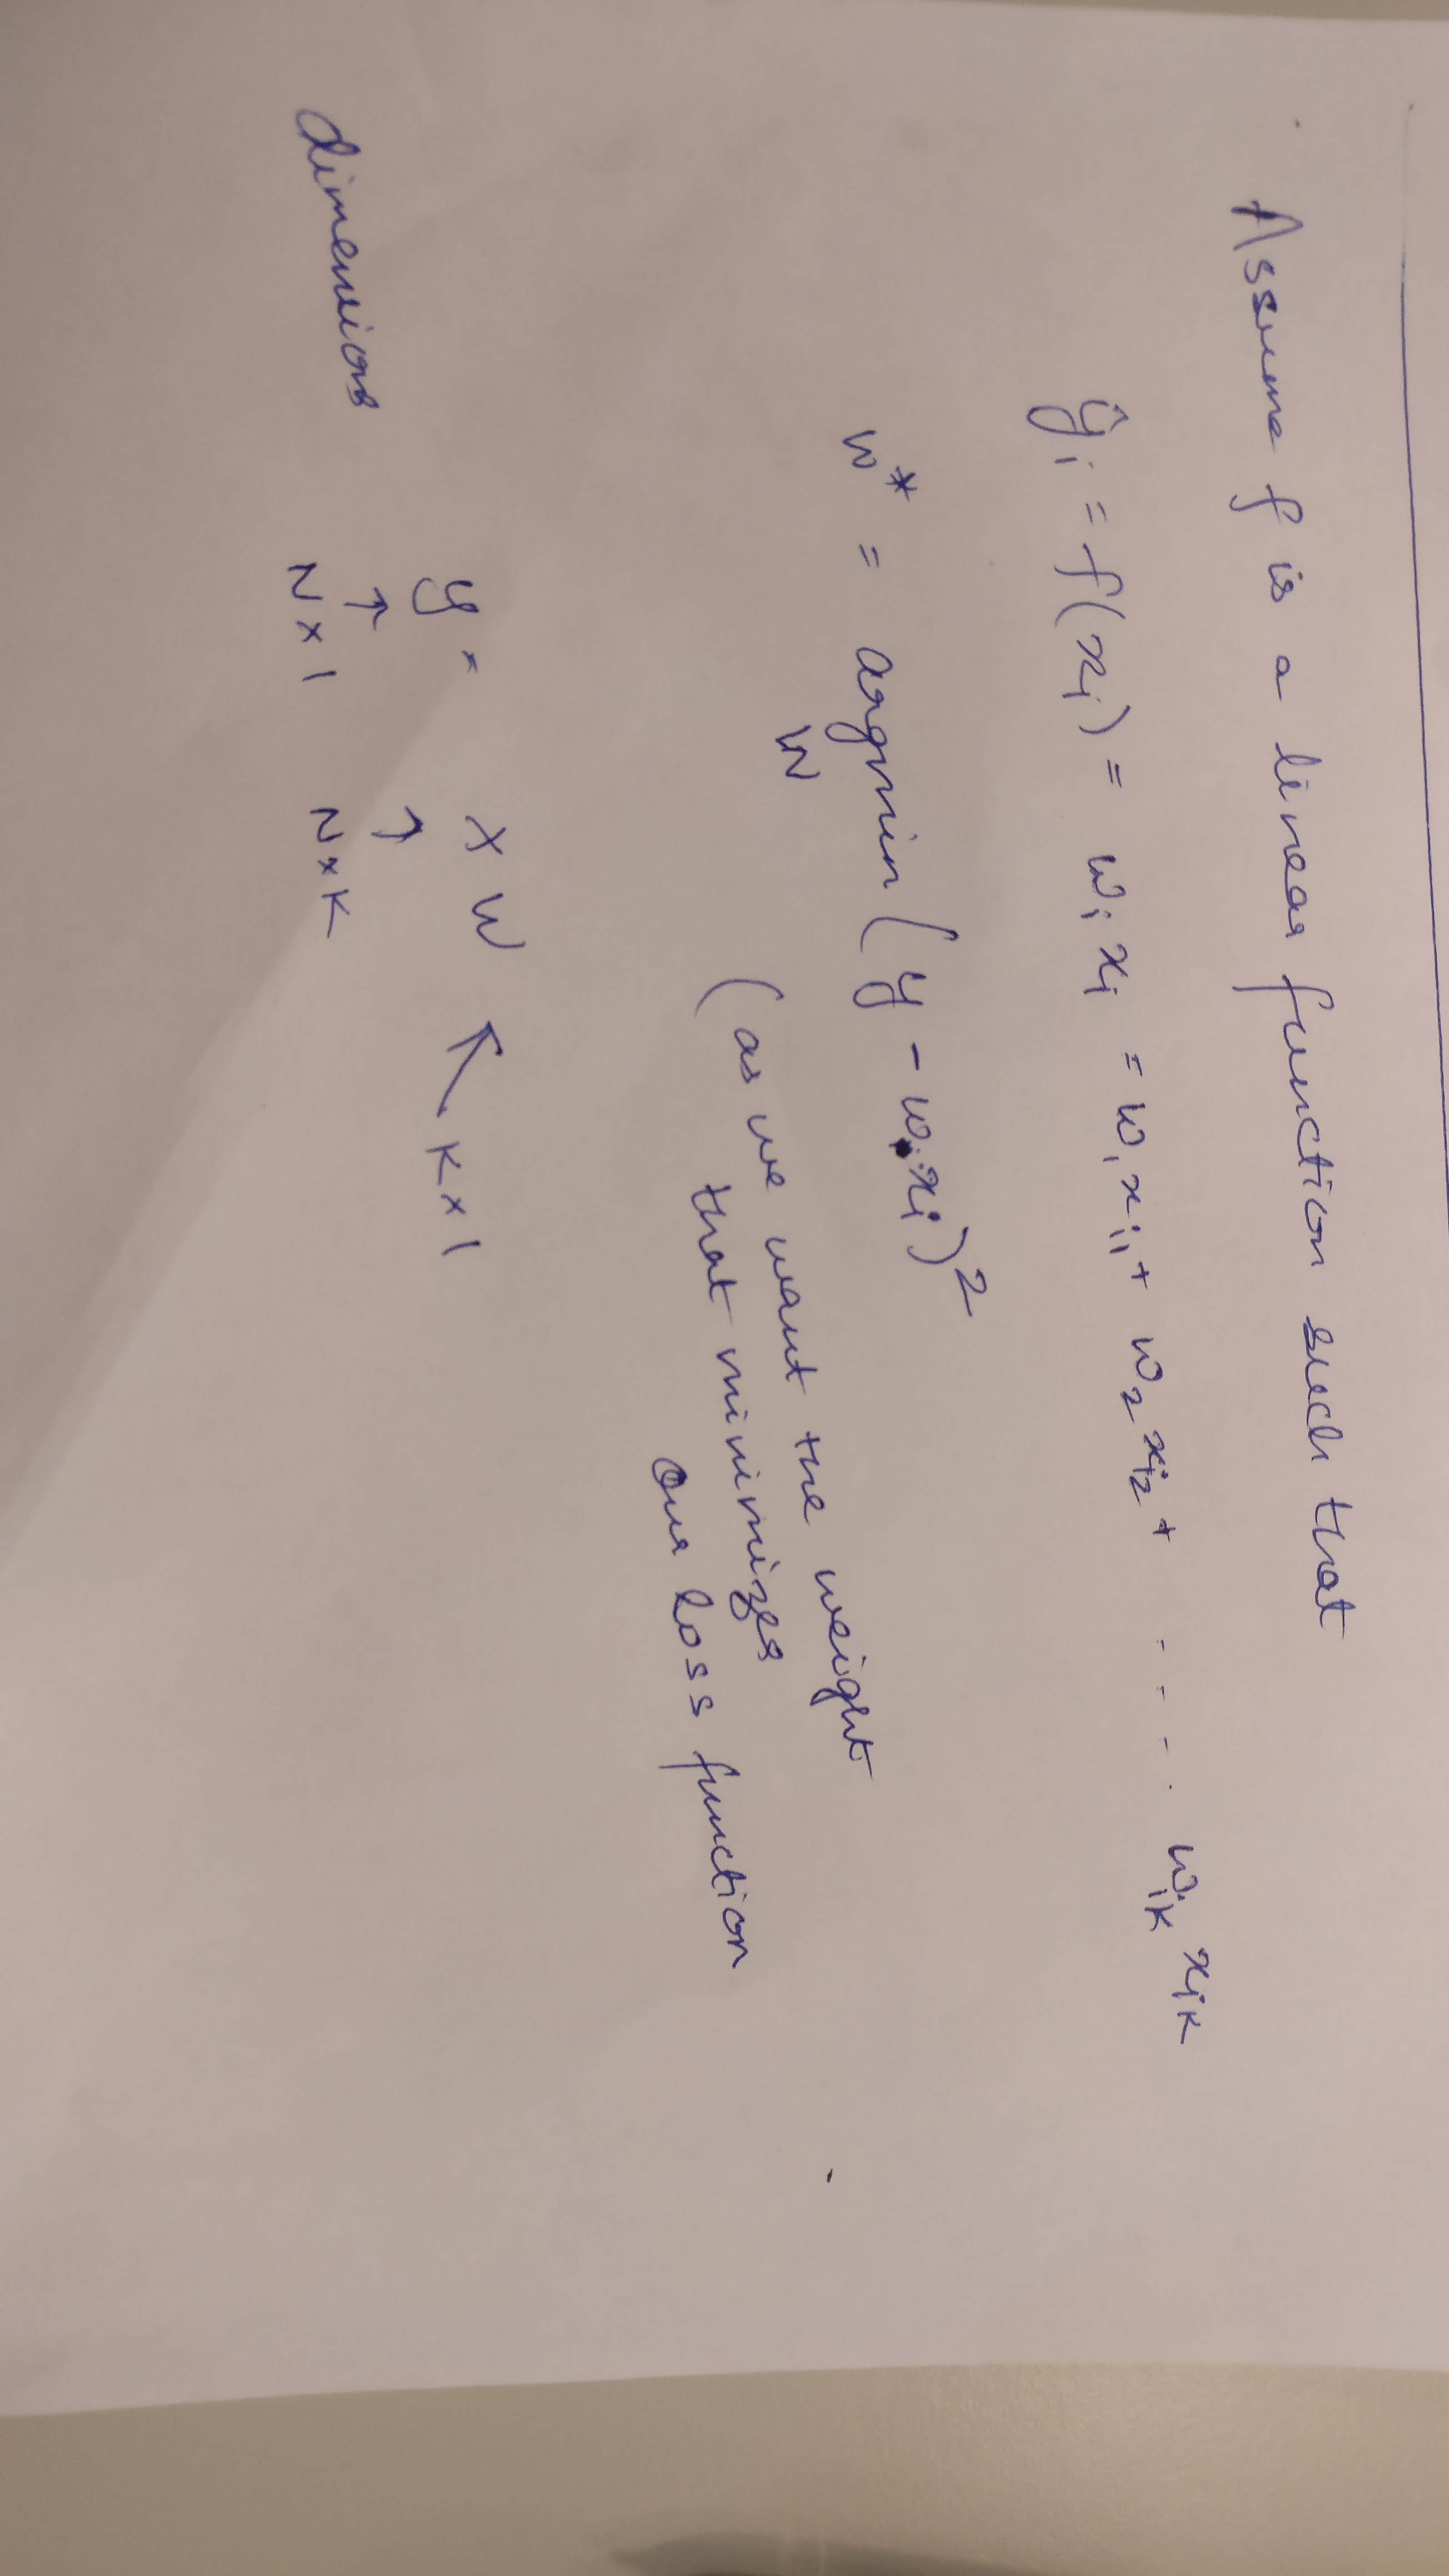
\includegraphics[width=8cm,height = 10cm, angle = 90, origin=c]{figures/compute_w_1.jpg}
\\
\\
Continued computation given on next page

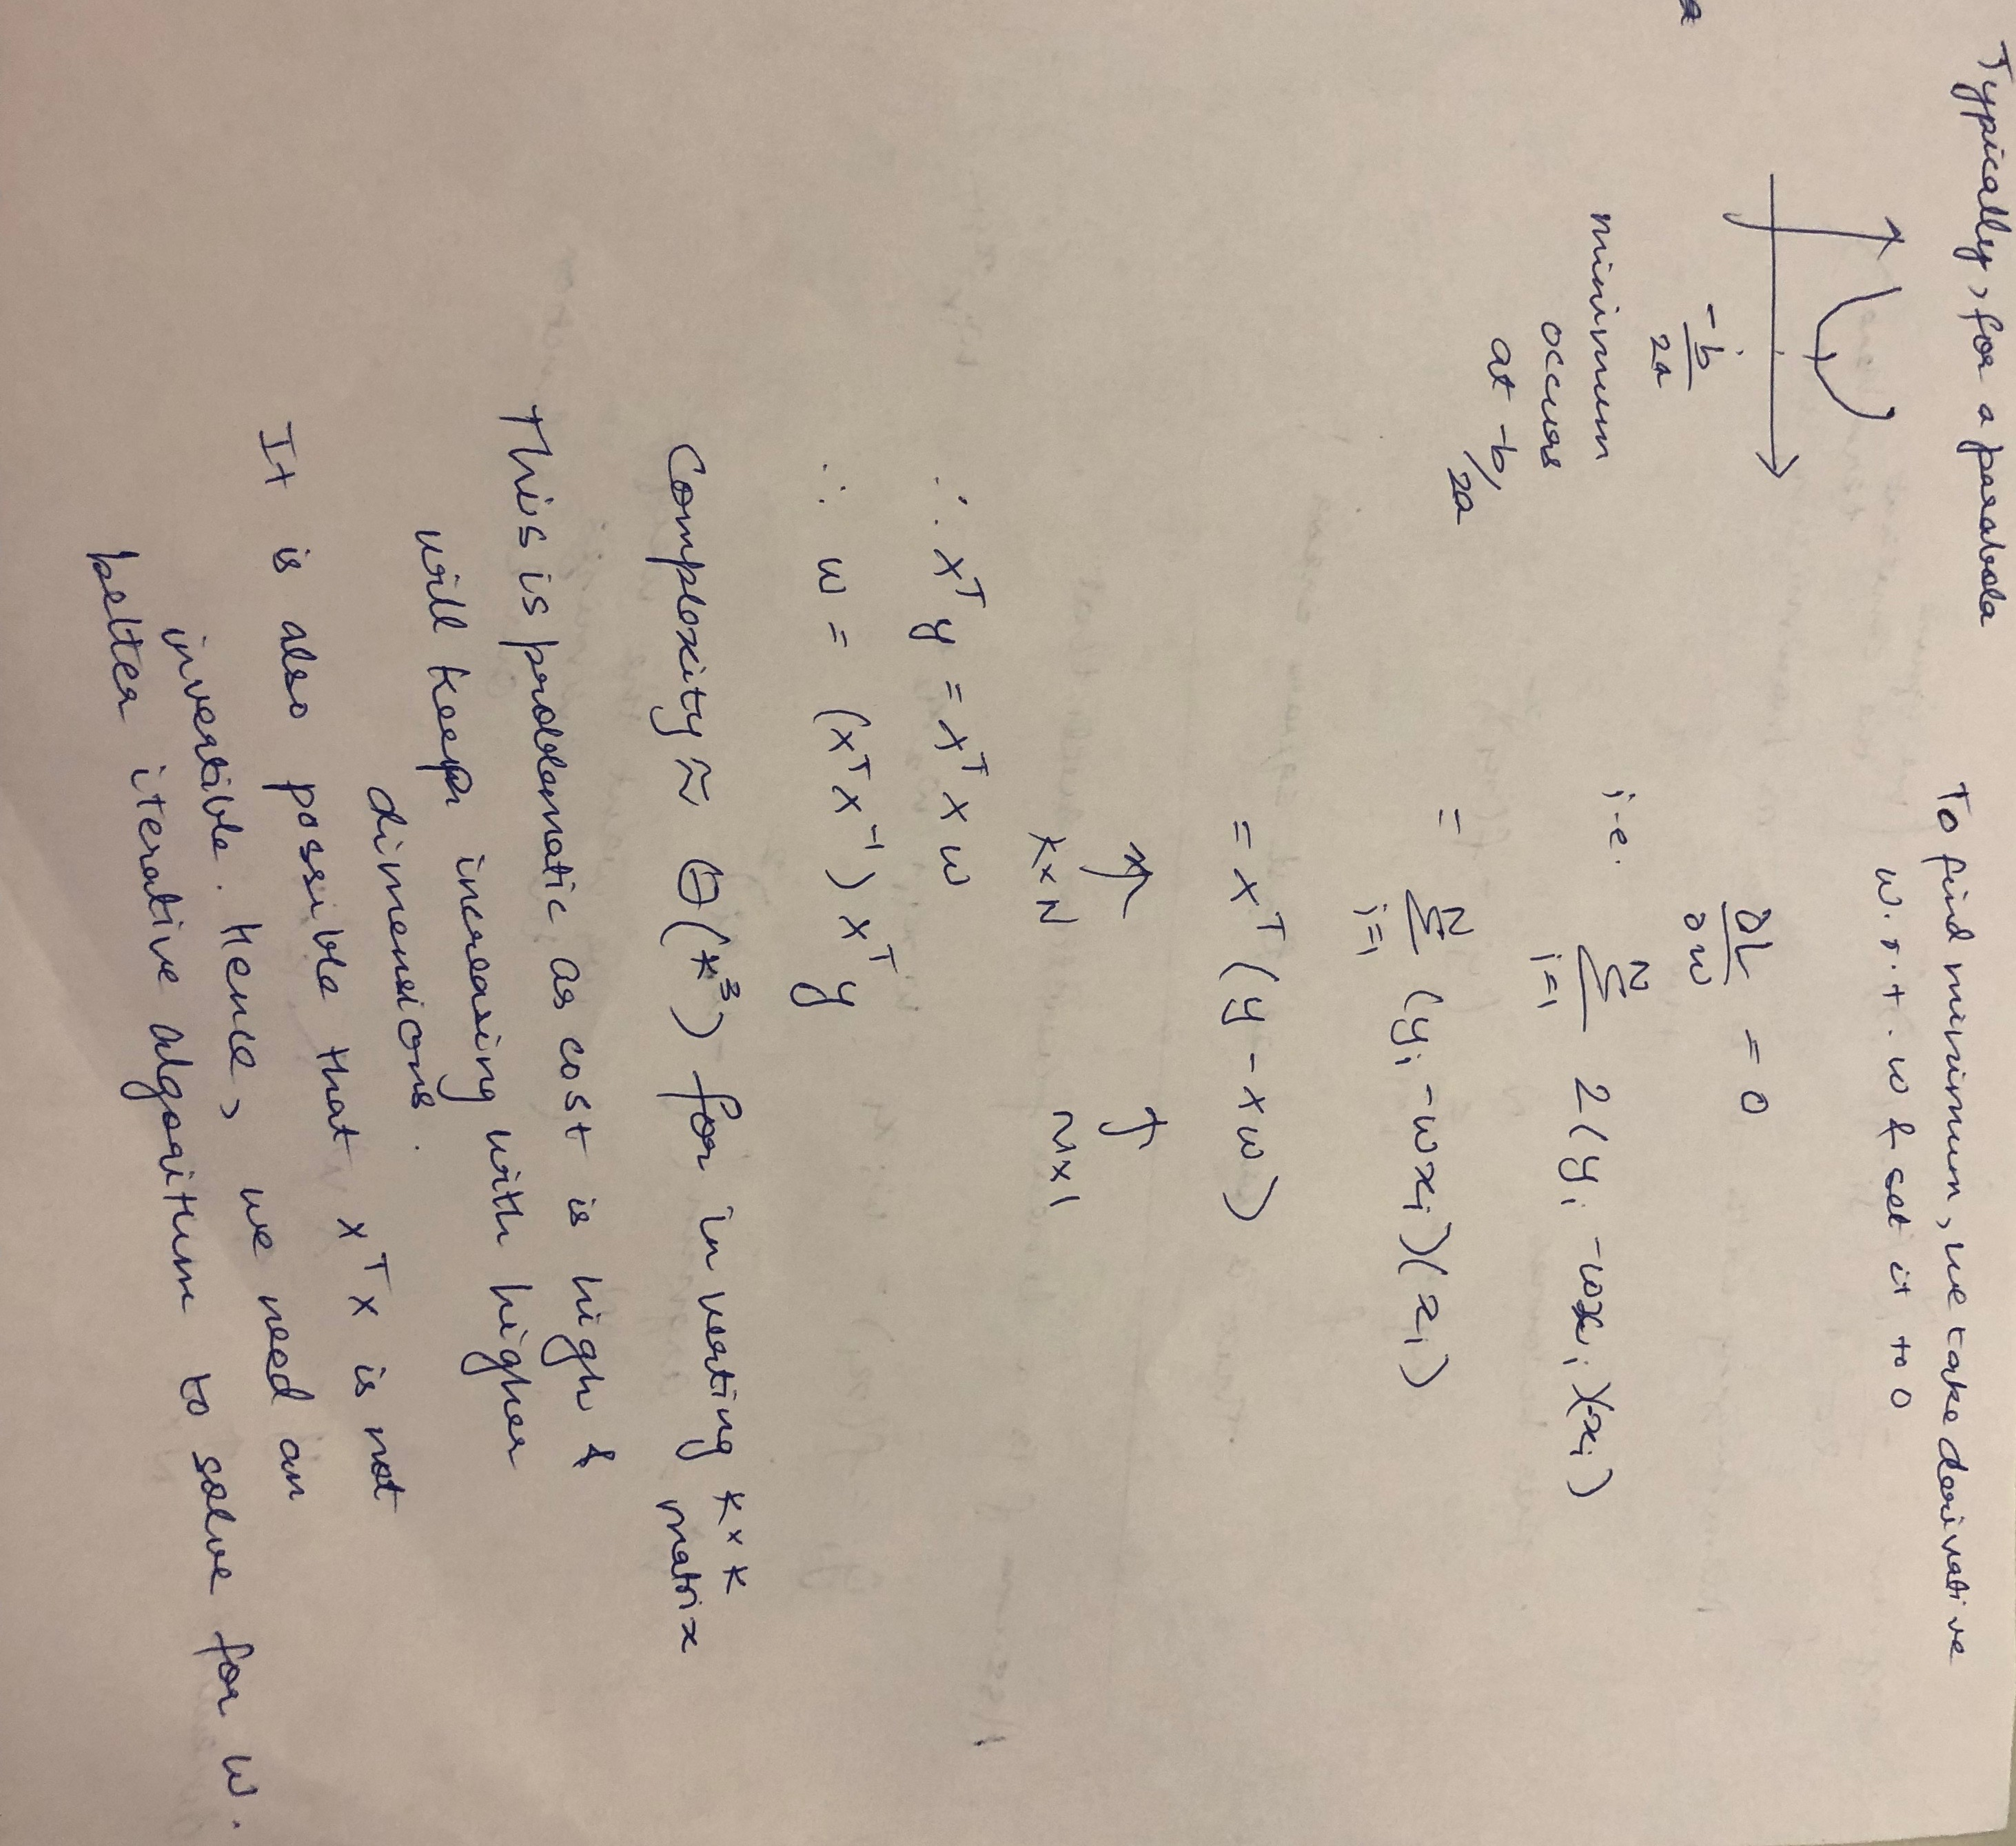
\includegraphics[width=15cm,height = 12cm, angle = 90, origin=c]{figures/compute_2.JPG}




\subsection{Gradient Descent}
We update weights as $$w := w - \alpha\frac{\partial L}{\partial w}$$
\\
where L is the loss function
\\
which is $$w := w - \alpha\frac{2}{N}X^T(y-Xw)$$ as the update rule at each step.
\\
\\
where $\alpha$ is called the learning rate, which is the step size we take at each iteration in the direction of negative gradient. This method take $O(kN)$ to compute the update for w at each step.
\\
\\
There are variations to this vanilla form of gradient descent-
One such variation is the stochastic gradient descent where we update w using a smaller batch size (or 1 data point)
$$w := w - \alpha(y_i - w \cdot x_i)x_i$$ 
\\
This method only requires $O(mK)$ where m is the batch size


\end{document}

%%% Local Variables:
%%% mode: latex
%%% TeX-master: t
%%% End:
